\documentclass[fleqn]{jbook}
\usepackage{physpub}
\usepackage{txfonts}

\begin{document}
\begin{question}{問題4}{高山 務}
\begin{enumerate}
\item
半径$a$、厚さ$d(\ll a)$、一様な密度$\rho$の薄い円盤の、中心を通り面に垂直な軸のまわりの慣性モーメント$I_z$、および中心を通り面に平行な軸のまわりの慣性モーメント$I_x$を求めよ。
\item
半径$a$、質量$M$の一様な球の、質量中心を通る軸のまわりの慣性モーメントが
\begin{eqnarray}
I=\frac{2}{5}Ma^2
\end{eqnarray}
であることを示せ。
\item
この球を摩擦のある水平な面に置き、中心の高さを中心に向かって水平に突いて初速$v_0$を与えた。球と面の静止摩擦係数を$\mu$、動摩擦係数を$\mu'$とするとき、球が滑らずに転がるようになるまでの時間と、それまでに質量中心が進む距離を求めよ。また滑らずに転がるようになってからの質量中心の速さ$v$と回転の角速度$\omega$を求めよ。ただし、以下の設問も含め、転がり摩擦は無視するものとする。
\item
図1のように、面が前方で傾斜角$\theta$の上り斜面になっているとする。$\theta$がある値より大きいと、滑らずに転がってきた球は滑りながら斜面を上るようになる。その$\theta$の値を求めよ。ただし、斜面の下端は図1のように十分短い範囲で緩やかに変化しており、斜面全体にわたって摩擦係数は水平な部分と同じであるとする。
\begin{figure}[htbp]
\begin{center}
%\includegraphics[width=.6\linewidth]{2002phy4q.eps}
\includegraphics[width=.6\linewidth]{2002physQ4_1.eps}
\end{center}
\end{figure}
\item
前方の斜面の部分に摩擦があり球が滑らずに転がって上る場合と、斜面の部分が滑らかで摩擦がない場合では、球はどちらが高くまで上ることができるか。理由を付けて答えよ。
\end{enumerate}
\end{question}

\begin{answer}{問題4}{高山 務}
\setcounter{equation}{0}
\begin{enumerate}
\item
慣性モーメント$I$は、軸からの距離を$r$として、
\begin{eqnarray}
I=\int_V d^3 r r^2 \rho
\end{eqnarray}
と表される。

従って、中心を通り面に垂直な軸を取った場合の円盤の慣性モーメント$I_z$は、円盤の面上での中心からの距離を$r$、回転角を$\theta$、厚さの方向を$z$として表した円柱座標$(r,\theta,z)$を用いて
\begin{eqnarray}
I_z = \int_0^d dz \int_0^a dr \int_0^{2\pi} d\theta r r^2 \rho = 2 \pi \rho \int_0^a r^3 = \frac{1}{2}\pi \rho d a^4
\end{eqnarray}

一方、中心を通り面に平行な軸を取った場合の慣性モーメント$I_x$は、中心を原点とし、軸を$x$軸、円盤の面を$xy$平面とした正規直交座標を用いて
\begin{eqnarray}
I_x &=& \int_{-a}^a dx \int_{-\frac{d}{2}}^{\frac{d}{2}} dy \int_{-\sqrt{a^2-x^2}}^{\sqrt{a^2-x^2}} dz (z^2 + y^2)\rho = \frac{1}{4}\pi\rho da^4+\frac{1}{12}\pi\rho d^3a^2
\end{eqnarray}
$d<<a$として小さな項を無視すれば
\begin{eqnarray}
I_x = \frac{1}{4}\pi\rho da^4
\end{eqnarray}
となる。
\item
極座標で計算すると、中心軸からの距離は$r\sin\theta$となる。

また、球が一様であれば、密度$\rho$は$\displaystyle \rho=\frac{3M}{4\pi a^3}$によって与えられる。

この$\rho$を用いて、慣性モーメント$I$は
\begin{eqnarray}
I=\int_0^a dr \int_{-1}^1 d(\cos\theta) \int_0^{2\pi} d\phi r^2 r^2 \sin^2\theta = 2\pi \rho \Bigl(1-\frac{2}{3} \Bigl) \int_0^a dr r^4 = \frac{8}{15}\pi \rho a^5
\end{eqnarray}

$\rho$を代入すると、
\begin{eqnarray}
I=\frac{2}{5}Ma^2
\end{eqnarray}
が得られる。
\item
運動を始めた球は摩擦力を受けながら運動し、並進運動の速度$v$が回転の速度$a\omega$と等しくなったときに、球の面との接点が面に対して静止する。これ以降は球は転がって運動し始め、摩擦が働かなくなって\footnote{球と面の接点は常に面に対して静止}一定の速度および角速度で運動するようになる。

球が滑っているとき、接点で働く摩擦力の大きさは、球を支える垂直抗力が$Mg$であることから$Mg\mu'$であり、初速による球の進行方向と逆向きに働く。

\begin{minipage}{.7\linewidth}
運動方程式を立てると、並進運動の速度$v$については
\begin{eqnarray}
M\frac{dv}{dt} = -Mg\mu'
\end{eqnarray}

回転については、正の向きの回転によって球がはじめの進行方向と同じ向きに進むように$\omega$の正の方向を取って
\begin{eqnarray}
I\frac{d\omega}{dt} = Mg\mu' a
\end{eqnarray}
$I$は慣性モーメントであり、前の問題より$\displaystyle I=\frac{2}{5}Ma^2$である。\end{minipage}
\begin{minipage}{.3\linewidth}
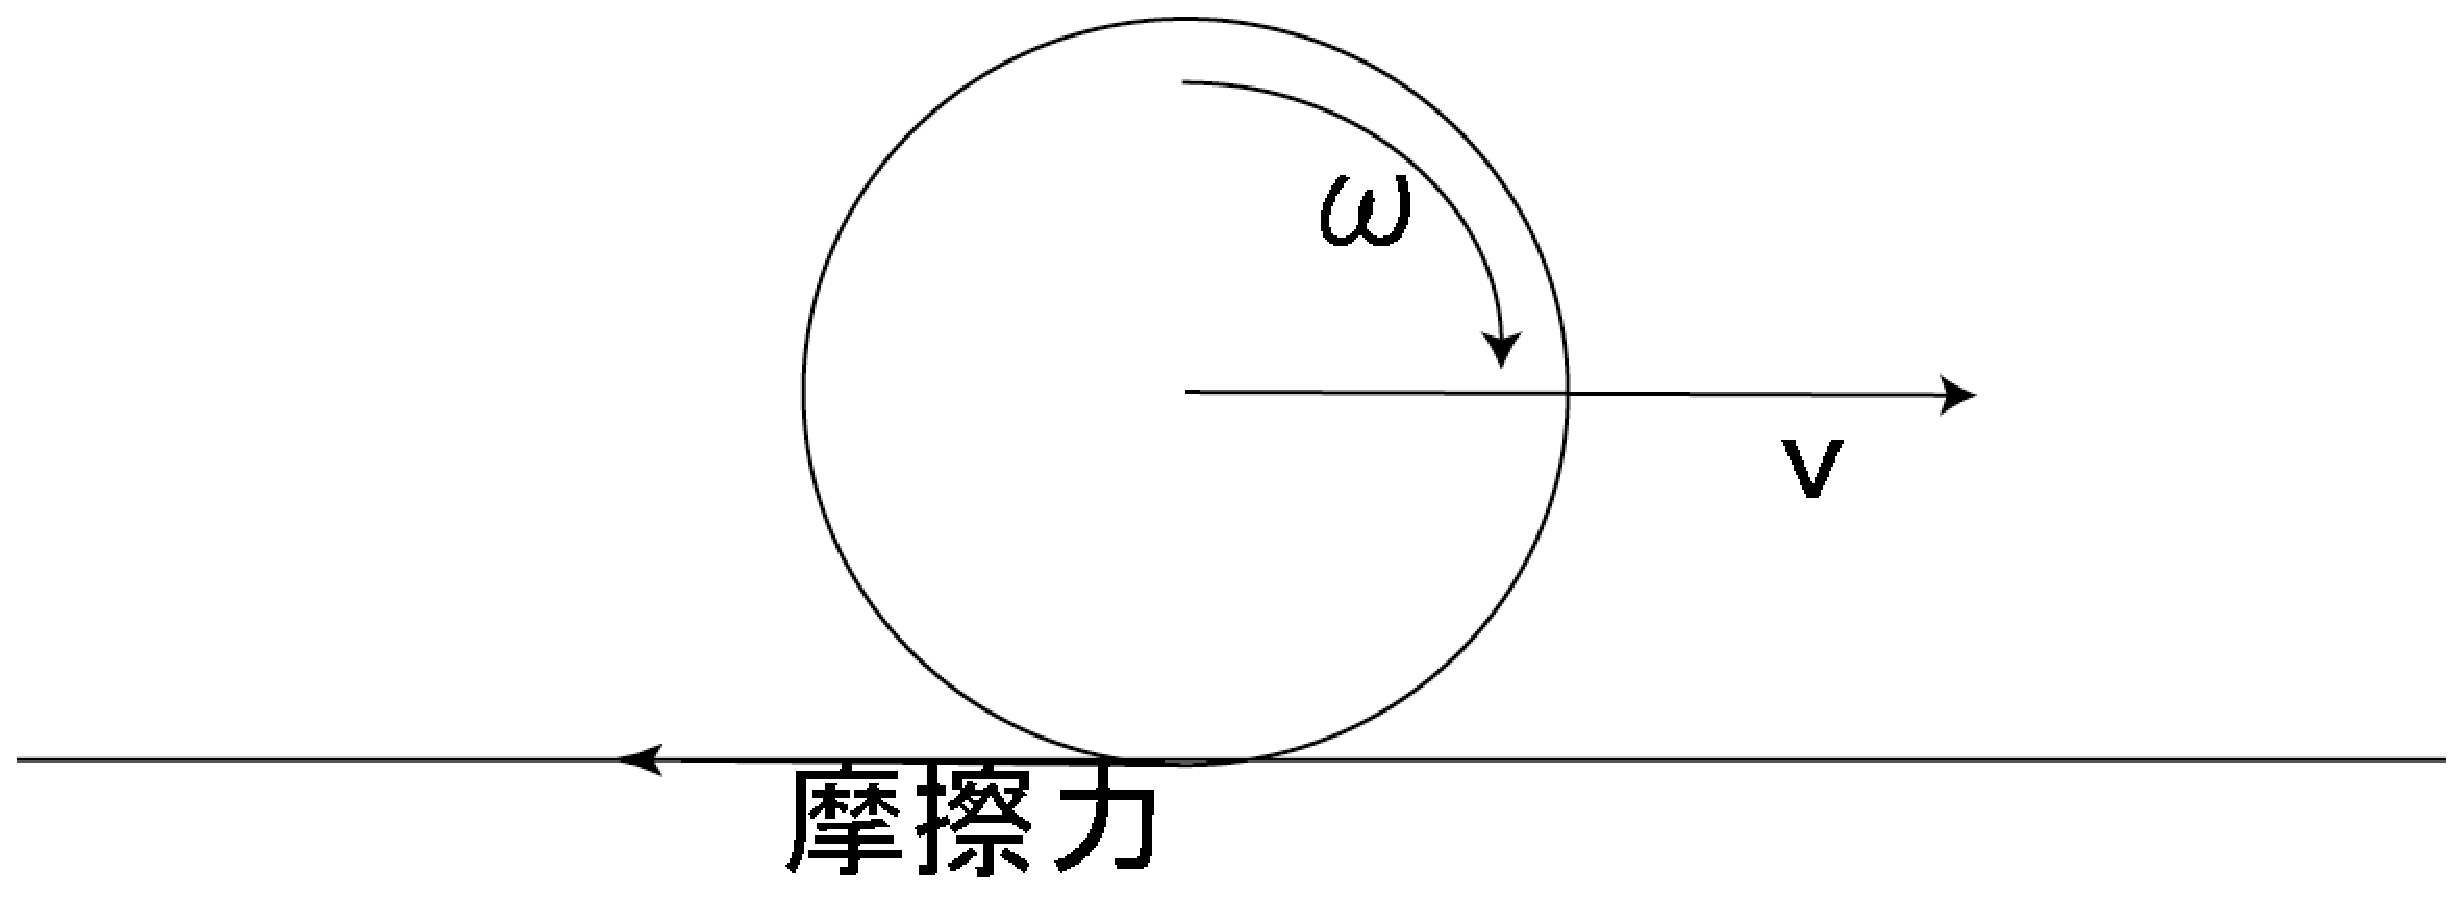
\includegraphics[width=\linewidth]{2002phy4a1.eps}
\end{minipage}

初期条件$v=v_0,\omega=0$から、球の運動は
\begin{eqnarray}
v &=& v_0-Mg\mu' t \\
\omega &=& \frac{5g\mu'}{2a}t
\end{eqnarray}
に従う。

回転を始めるときの条件$v=a\omega$より、このときの時刻を求めると
\begin{eqnarray}
t=\frac{2v_0}{7g\mu'}
\end{eqnarray}
このときの速度および角速度は、
\begin{eqnarray}
v=\frac{5}{7}v_0 ~,~ \omega=\frac{5v_0}{7a}
\end{eqnarray}
\item
球が坂を上り始めると、重力および接点での摩擦力に従って運動し始める。

\begin{minipage}{.7\linewidth}
坂を上る方向の速度を$v$、球が坂を上る方向に運動するような回転の方向を$\omega$と取り直す。

斜面の下端は十分短い範囲で緩やかに変化しているため、球は問3で求めた速度および角速度を保ったまま斜面を上り始めると考えて良い。

坂を上る方向を力の正の向きにとって、摩擦力を$f$として表すと、球の速度及び角速度が従う運動方程式は
\begin{eqnarray}
M\frac{dv}{dt} &=& -Mg\sin\theta + f \\
I\frac{d\omega}{dt} &=& - af 
\end{eqnarray}
によって与えられる。
\end{minipage}
\begin{minipage}{.3\linewidth}
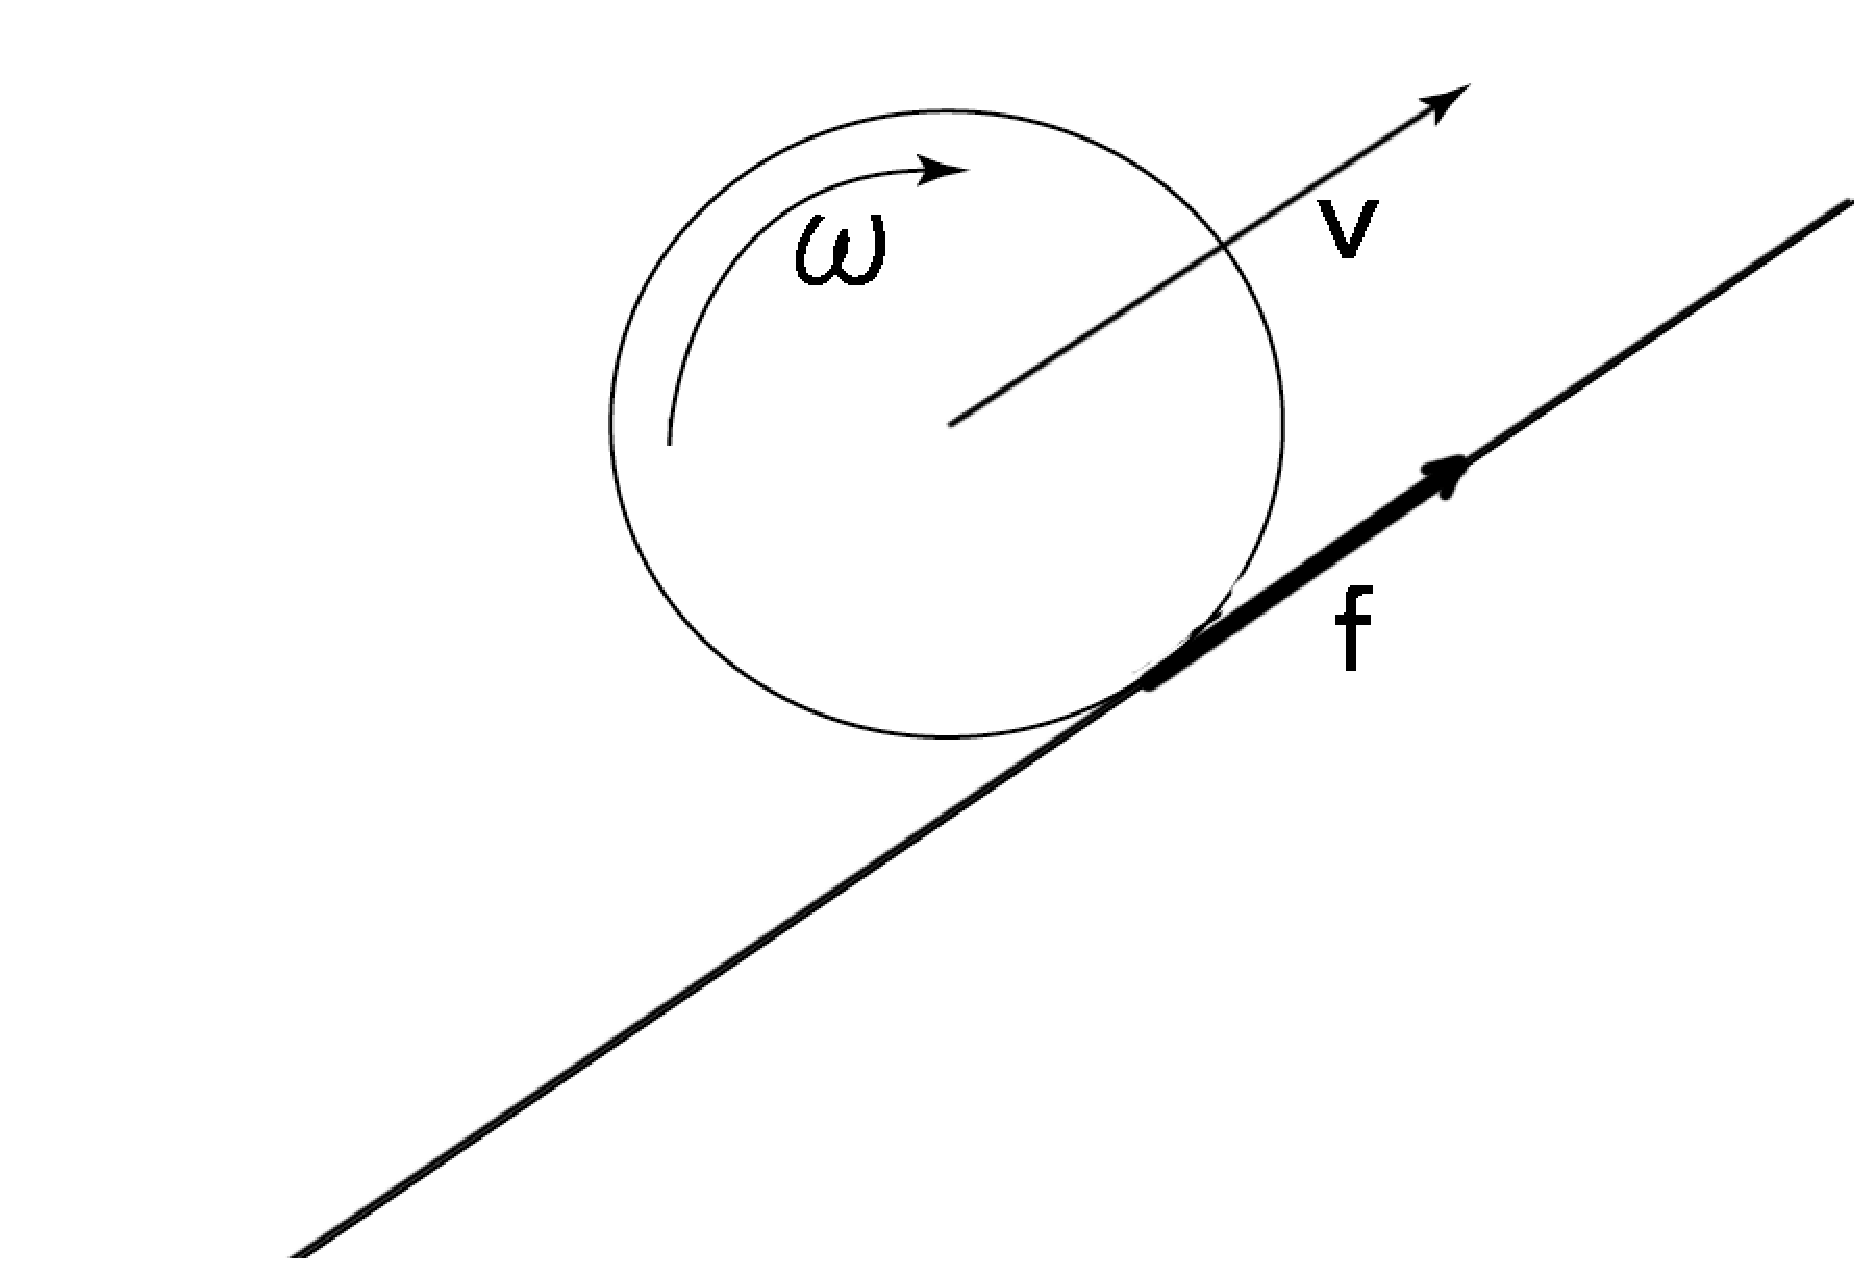
\includegraphics[width=\linewidth]{2002phy4a2.eps}
\end{minipage}

重力は球全体に一様に働き、垂直抗力は球の中心に向かって働くので、これらによるモーメントは考えなくて良い。

球に働く垂直抗力が$Mg\cos\theta$であるから、$f$は最大で$Mg\mu\cos\theta$までの大きさを取る。

斜面が緩やかであれば、球は接点が面に対して静止し続ける条件$v=a\omega$を満たすように運動し、転がったまま斜面を上る。このとき、$\dot{v}=a\dot{\omega}$を満たすので、$f$は
\begin{eqnarray}
- \frac{a^2 f}{I} = -g\sin\theta+\frac{f}{m} \nonumber
\end{eqnarray}
即ち
\begin{eqnarray}
\ilabel{friction}
f=\frac{2Mg}{7}\sin\theta
\end{eqnarray}
を満たす。

斜面が急な場合、$f$の最大の条件から式(\iref{friction})を満たすような$f$が存在しなくなると、球の接点は面に対して静止できずに滑り出すことになる。

従って、球が滑り出すような最小の$\theta$は
\begin{eqnarray}
Mg\mu\cos\theta = \frac{2Mg}{7}\sin\theta
\end{eqnarray}
によって与えられる。$\theta$を計算すると、
\begin{eqnarray}
\theta=\arctan\Bigl( \frac{7\mu}{2} \Bigl)
\end{eqnarray}
この場合、摩擦力は$f=Mg\mu\cos\theta$となり、$\dot{v}<a\dot{\omega}$となって球は空回りし始める。滑り出した後は$f=Mg\mu' \cos\theta<Mg\mu\cos\theta$より$\dot{v}<a\dot{\omega}$の関係が続くため、球は空回りし続けることになる。
\item
球が最大の高さまで上ったとき、並進運動速度$v$は0となる。

摩擦があって球が滑らずに上る場合、$v=a\omega$より、最大の高さまで上った時点で$v=\omega=0$となって、球の運動エネルギーは0になる。転がって運動している限り摩擦力は仕事をしないので、系の力学的エネルギーは保存されている。従って、この場合、斜面を上り始めたときの球の全運動エネルギーと等しい位置エネルギーを得る高さまで球は斜面を上ることができる。

一方、摩擦がない場合、球にモーメントは働かないので回転は止まらず、最大の高さまで上った時点でも球は運動エネルギーを持つ。このときの位置エネルギーは斜面を上り始めたときの球の全運動エネルギーよりも低い。

以上より、摩擦がある場合の方が球は高い位置まで上ることができる。
\end{enumerate}
\end{answer}
\end{document}
